\documentclass{standalone}
\usepackage{tikz}
\usetikzlibrary{patterns, positioning}


\begin{document}
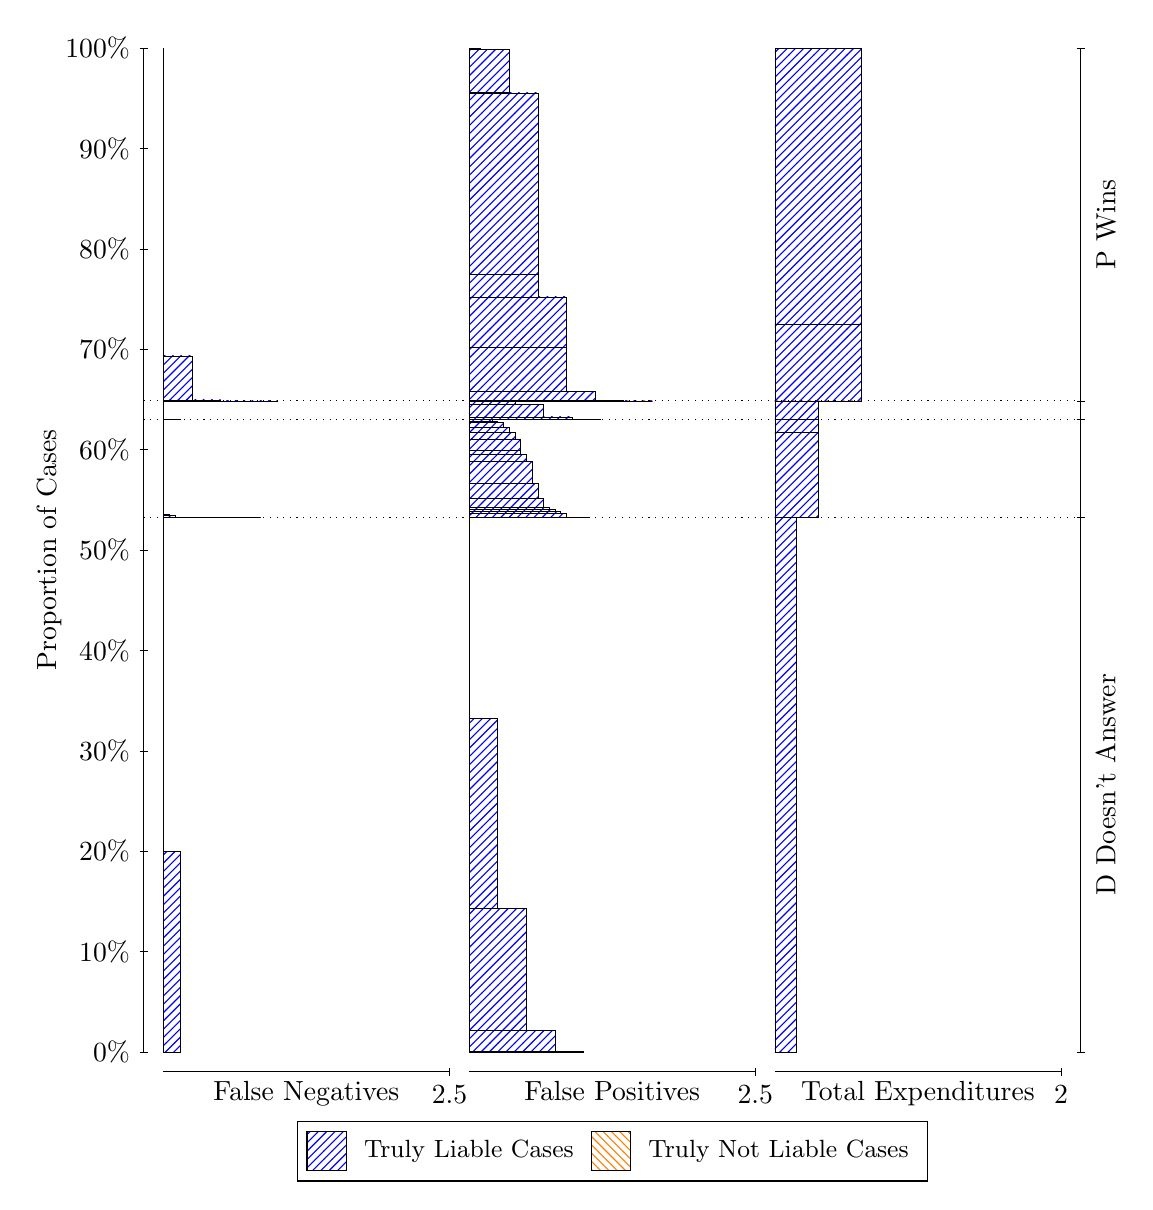
\begin{tikzpicture}
\draw[black, very thin] (1.5,1.75) -- (1.5,14.5);
\node[rotate=90, text=black, anchor=center] at (0.3, 8.125) {Proportion of Cases};
\draw[black, very thin] (1.45,1.75) -- (1.55,1.75);
\node[text=black, anchor=east] at (1.45, 1.75) {0\%};
\draw[black, very thin] (1.45,3.025) -- (1.55,3.025);
\node[text=black, anchor=east] at (1.45, 3.025) {10\%};
\draw[black, very thin] (1.45,4.3) -- (1.55,4.3);
\node[text=black, anchor=east] at (1.45, 4.3) {20\%};
\draw[black, very thin] (1.45,5.575) -- (1.55,5.575);
\node[text=black, anchor=east] at (1.45, 5.575) {30\%};
\draw[black, very thin] (1.45,6.85) -- (1.55,6.85);
\node[text=black, anchor=east] at (1.45, 6.85) {40\%};
\draw[black, very thin] (1.45,8.125) -- (1.55,8.125);
\node[text=black, anchor=east] at (1.45, 8.125) {50\%};
\draw[black, very thin] (1.45,9.4) -- (1.55,9.4);
\node[text=black, anchor=east] at (1.45, 9.4) {60\%};
\draw[black, very thin] (1.45,10.675) -- (1.55,10.675);
\node[text=black, anchor=east] at (1.45, 10.675) {70\%};
\draw[black, very thin] (1.45,11.95) -- (1.55,11.95);
\node[text=black, anchor=east] at (1.45, 11.95) {80\%};
\draw[black, very thin] (1.45,13.225) -- (1.55,13.225);
\node[text=black, anchor=east] at (1.45, 13.225) {90\%};
\draw[black, very thin] (1.45,14.5) -- (1.55,14.5);
\node[text=black, anchor=east] at (1.45, 14.5) {100\%};

\draw[black, very thin] (13.4,1.75) -- (13.4,14.5);
\draw[black, very thin] (13.35,1.75) -- (13.45,1.75);
\node[anchor=west] at (13.35, 1.75) {};
\draw[black, very thin] (13.35,8.5362) -- (13.45,8.5362);
\node[anchor=west] at (13.35, 8.5362) {};
\draw[black, very thin] (13.35,9.7863) -- (13.45,9.7863);
\node[anchor=west] at (13.35, 9.7863) {};
\draw[black, very thin] (13.35,10.019) -- (13.45,10.019);
\node[anchor=west] at (13.35, 10.019) {};
\draw[black, very thin] (13.35,14.5) -- (13.45,14.5);
\node[anchor=west] at (13.35, 14.5) {};

\draw[black, very thin, pattern color=blue, pattern=north east lines] (1.75,1.75) rectangle (1.968,4.2985);
\draw[black, very thin, pattern color=orange, pattern=north west lines] (1.75,4.2985) rectangle (1.75,4.2985);
\draw[black, very thin, pattern color=blue, pattern=north east lines] (1.75,4.2985) rectangle (1.75,8.5362);
\draw[black, very thin, pattern color=blue, pattern=north east lines] (1.75,8.5362) rectangle (2.9853,8.5362);
\draw[black, very thin, pattern color=blue, pattern=north east lines] (1.75,8.5362) rectangle (2.84,8.5362);
\draw[black, very thin, pattern color=blue, pattern=north east lines] (1.75,8.5362) rectangle (2.6947,8.5362);
\draw[black, very thin, pattern color=blue, pattern=north east lines] (1.75,8.5362) rectangle (2.622,8.5362);
\draw[black, very thin, pattern color=blue, pattern=north east lines] (1.75,8.5362) rectangle (2.5493,8.5362);
\draw[black, very thin, pattern color=blue, pattern=north east lines] (1.75,8.5362) rectangle (2.4767,8.5362);
\draw[black, very thin, pattern color=blue, pattern=north east lines] (1.75,8.5362) rectangle (2.404,8.5362);
\draw[black, very thin, pattern color=blue, pattern=north east lines] (1.75,8.5362) rectangle (2.3313,8.5362);
\draw[black, very thin, pattern color=blue, pattern=north east lines] (1.75,8.5362) rectangle (2.2587,8.5363);
\draw[black, very thin, pattern color=blue, pattern=north east lines] (1.75,8.5363) rectangle (2.186,8.5364);
\draw[black, very thin, pattern color=blue, pattern=north east lines] (1.75,8.5364) rectangle (2.1133,8.537);
\draw[black, very thin, pattern color=blue, pattern=north east lines] (1.75,8.537) rectangle (2.0407,8.5382);
\draw[black, very thin, pattern color=blue, pattern=north east lines] (1.75,8.5382) rectangle (1.968,8.5433);
\draw[black, very thin, pattern color=blue, pattern=north east lines] (1.75,8.5433) rectangle (1.8953,8.5618);
\draw[black, very thin, pattern color=blue, pattern=north east lines] (1.75,8.5618) rectangle (1.8953,8.5637);
\draw[black, very thin, pattern color=blue, pattern=north east lines] (1.75,8.5637) rectangle (1.8227,8.5733);
\draw[black, very thin, pattern color=orange, pattern=north west lines] (1.75,8.5733) rectangle (1.75,8.5733);
\draw[black, very thin, pattern color=blue, pattern=north east lines] (1.75,8.5733) rectangle (1.75,9.7863);
\draw[black, very thin, pattern color=blue, pattern=north east lines] (1.75,9.7863) rectangle (1.968,9.7867);
\draw[black, very thin, pattern color=orange, pattern=north west lines] (1.75,9.7867) rectangle (1.75,9.7867);
\draw[black, very thin, pattern color=blue, pattern=north east lines] (1.75,9.7867) rectangle (1.75,10.019);
\draw[black, very thin, pattern color=blue, pattern=north east lines] (1.75,10.019) rectangle (3.2033,10.019);
\draw[black, very thin, pattern color=blue, pattern=north east lines] (1.75,10.019) rectangle (2.84,10.019);
\draw[black, very thin, pattern color=blue, pattern=north east lines] (1.75,10.019) rectangle (2.4767,10.032);
\draw[black, very thin, pattern color=blue, pattern=north east lines] (1.75,10.032) rectangle (2.1133,10.589);
\draw[black, very thin, pattern color=orange, pattern=north west lines] (1.75,10.589) rectangle (1.75,10.589);
\draw[black, very thin, pattern color=blue, pattern=north east lines] (1.75,10.589) rectangle (1.75,14.5);
\draw[black, very thin, pattern color=orange, pattern=north west lines] (5.6333,1.75) rectangle (7.0867,1.75);
\draw[black, very thin, pattern color=blue, pattern=north east lines] (5.6333,1.75) rectangle (7.0867,1.7527);
\draw[black, very thin, pattern color=blue, pattern=north east lines] (5.6333,1.7527) rectangle (6.7233,2.0217);
\draw[black, very thin, pattern color=blue, pattern=north east lines] (5.6333,2.0217) rectangle (6.36,3.5772);
\draw[black, very thin, pattern color=blue, pattern=north east lines] (5.6333,3.5772) rectangle (5.9967,5.9877);
\draw[black, very thin, pattern color=blue, pattern=north east lines] (5.6333,5.9877) rectangle (5.6333,8.5362);
\draw[black, very thin, pattern color=orange, pattern=north west lines] (5.6333,8.5362) rectangle (7.1593,8.5362);
\draw[black, very thin, pattern color=blue, pattern=north east lines] (5.6333,8.5362) rectangle (7.1593,8.5363);
\draw[black, very thin, pattern color=orange, pattern=north west lines] (5.6333,8.5363) rectangle (7.014,8.5363);
\draw[black, very thin, pattern color=blue, pattern=north east lines] (5.6333,8.5363) rectangle (7.014,8.5365);
\draw[black, very thin, pattern color=orange, pattern=north west lines] (5.6333,8.5365) rectangle (6.8687,8.5365);
\draw[black, very thin, pattern color=blue, pattern=north east lines] (5.6333,8.5365) rectangle (6.8687,8.5899);
\draw[black, very thin, pattern color=blue, pattern=north east lines] (5.6333,8.5899) rectangle (6.796,8.6168);
\draw[black, very thin, pattern color=orange, pattern=north west lines] (5.6333,8.6168) rectangle (6.7233,8.6168);
\draw[black, very thin, pattern color=blue, pattern=north east lines] (5.6333,8.6168) rectangle (6.7233,8.6447);
\draw[black, very thin, pattern color=blue, pattern=north east lines] (5.6333,8.6447) rectangle (6.6507,8.662);
\draw[black, very thin, pattern color=orange, pattern=north west lines] (5.6333,8.662) rectangle (6.578,8.662);
\draw[black, very thin, pattern color=blue, pattern=north east lines] (5.6333,8.662) rectangle (6.578,8.7757);
\draw[black, very thin, pattern color=blue, pattern=north east lines] (5.6333,8.7757) rectangle (6.5053,8.9676);
\draw[black, very thin, pattern color=orange, pattern=north west lines] (5.6333,8.9676) rectangle (6.4327,8.9676);
\draw[black, very thin, pattern color=blue, pattern=north east lines] (5.6333,8.9676) rectangle (6.4327,9.2515);
\draw[black, very thin, pattern color=blue, pattern=north east lines] (5.6333,9.2515) rectangle (6.36,9.3412);
\draw[black, very thin, pattern color=blue, pattern=north east lines] (5.6333,9.3412) rectangle (6.2873,9.3885);
\draw[black, very thin, pattern color=orange, pattern=north west lines] (5.6333,9.3885) rectangle (6.2873,9.3885);
\draw[black, very thin, pattern color=blue, pattern=north east lines] (5.6333,9.3885) rectangle (6.2873,9.5373);
\draw[black, very thin, pattern color=blue, pattern=north east lines] (5.6333,9.5373) rectangle (6.2147,9.6188);
\draw[black, very thin, pattern color=blue, pattern=north east lines] (5.6333,9.6188) rectangle (6.142,9.6792);
\draw[black, very thin, pattern color=blue, pattern=north east lines] (5.6333,9.6792) rectangle (6.0693,9.7492);
\draw[black, very thin, pattern color=blue, pattern=north east lines] (5.6333,9.7492) rectangle (5.9967,9.7587);
\draw[black, very thin, pattern color=blue, pattern=north east lines] (5.6333,9.7587) rectangle (5.924,9.7606);
\draw[black, very thin, pattern color=blue, pattern=north east lines] (5.6333,9.7606) rectangle (5.924,9.7792);
\draw[black, very thin, pattern color=blue, pattern=north east lines] (5.6333,9.7792) rectangle (5.8513,9.7843);
\draw[black, very thin, pattern color=blue, pattern=north east lines] (5.6333,9.7843) rectangle (5.7787,9.7855);
\draw[black, very thin, pattern color=blue, pattern=north east lines] (5.6333,9.7855) rectangle (5.706,9.7861);
\draw[black, very thin, pattern color=blue, pattern=north east lines] (5.6333,9.7861) rectangle (5.6333,9.7863);
\draw[black, very thin, pattern color=orange, pattern=north west lines] (5.6333,9.7863) rectangle (7.3047,9.7863);
\draw[black, very thin, pattern color=blue, pattern=north east lines] (5.6333,9.7863) rectangle (7.3047,9.7865);
\draw[black, very thin, pattern color=blue, pattern=north east lines] (5.6333,9.7865) rectangle (6.9413,9.8163);
\draw[black, very thin, pattern color=blue, pattern=north east lines] (5.6333,9.8163) rectangle (6.578,9.9771);
\draw[black, very thin, pattern color=blue, pattern=north east lines] (5.6333,9.9771) rectangle (6.2147,10.019);
\draw[black, very thin, pattern color=blue, pattern=north east lines] (5.6333,10.019) rectangle (5.8513,10.019);
\draw[black, very thin, pattern color=orange, pattern=north west lines] (5.6333,10.019) rectangle (7.9587,10.019);
\draw[black, very thin, pattern color=blue, pattern=north east lines] (5.6333,10.019) rectangle (7.9587,10.019);
\draw[black, very thin, pattern color=orange, pattern=north west lines] (5.6333,10.019) rectangle (7.5953,10.019);
\draw[black, very thin, pattern color=blue, pattern=north east lines] (5.6333,10.019) rectangle (7.5953,10.021);
\draw[black, very thin, pattern color=orange, pattern=north west lines] (5.6333,10.021) rectangle (7.232,10.021);
\draw[black, very thin, pattern color=blue, pattern=north east lines] (5.6333,10.021) rectangle (7.232,10.137);
\draw[black, very thin, pattern color=blue, pattern=north east lines] (5.6333,10.137) rectangle (6.8687,10.694);
\draw[black, very thin, pattern color=orange, pattern=north west lines] (5.6333,10.694) rectangle (6.8687,10.694);
\draw[black, very thin, pattern color=blue, pattern=north east lines] (5.6333,10.694) rectangle (6.8687,11.339);
\draw[black, very thin, pattern color=blue, pattern=north east lines] (5.6333,11.339) rectangle (6.5053,11.623);
\draw[black, very thin, pattern color=orange, pattern=north west lines] (5.6333,11.623) rectangle (6.5053,11.623);
\draw[black, very thin, pattern color=blue, pattern=north east lines] (5.6333,11.623) rectangle (6.5053,13.93);
\draw[black, very thin, pattern color=blue, pattern=north east lines] (5.6333,13.93) rectangle (6.142,13.94);
\draw[black, very thin, pattern color=blue, pattern=north east lines] (5.6333,13.94) rectangle (6.142,14.487);
\draw[black, very thin, pattern color=blue, pattern=north east lines] (5.6333,14.487) rectangle (5.7787,14.487);
\draw[black, very thin, pattern color=blue, pattern=north east lines] (5.6333,14.487) rectangle (5.7787,14.5);
\draw[black, very thin, pattern color=blue, pattern=north east lines] (5.6333,14.5) rectangle (5.6333,14.5);
\draw[black, very thin, pattern color=orange, pattern=north west lines] (9.5167,1.75) rectangle (9.7892,1.75);
\draw[black, very thin, pattern color=blue, pattern=north east lines] (9.5167,1.75) rectangle (9.7892,8.5362);
\draw[black, very thin, pattern color=orange, pattern=north west lines] (9.5167,8.5362) rectangle (10.062,8.5362);
\draw[black, very thin, pattern color=blue, pattern=north east lines] (9.5167,8.5362) rectangle (10.062,9.6188);
\draw[black, very thin, pattern color=orange, pattern=north west lines] (9.5167,9.6188) rectangle (10.062,9.6188);
\draw[black, very thin, pattern color=blue, pattern=north east lines] (9.5167,9.6188) rectangle (10.062,9.7863);
\draw[black, very thin, pattern color=orange, pattern=north west lines] (9.5167,9.7863) rectangle (10.062,9.7863);
\draw[black, very thin, pattern color=blue, pattern=north east lines] (9.5167,9.7863) rectangle (10.062,10.019);
\draw[black, very thin, pattern color=orange, pattern=north west lines] (9.5167,10.019) rectangle (10.607,10.019);
\draw[black, very thin, pattern color=blue, pattern=north east lines] (9.5167,10.019) rectangle (10.607,10.987);
\draw[black, very thin, pattern color=orange, pattern=north west lines] (9.5167,10.987) rectangle (10.607,10.987);
\draw[black, very thin, pattern color=blue, pattern=north east lines] (9.5167,10.987) rectangle (10.607,14.5);
\draw[black, dotted] (1.5,8.5362) -- (13.4,8.5362);
\draw[black, dotted] (1.5,9.7863) -- (13.4,9.7863);
\draw[black, dotted] (1.5,10.019) -- (13.4,10.019);
\draw[black, very thin] (1.75,1.5) -- (5.3833,1.5);
\node[text=black, anchor=north] at (3.5667, 1.5) {False Negatives};
\draw[black, very thin] (5.3833,1.45) -- (5.3833,1.55);
\node[text=black, anchor=north] at (5.3833, 1.45) {2.5};

\draw[black, very thin] (5.6333,1.5) -- (9.2667,1.5);
\node[text=black, anchor=north] at (7.45, 1.5) {False Positives};
\draw[black, very thin] (9.2667,1.45) -- (9.2667,1.55);
\node[text=black, anchor=north] at (9.2667, 1.45) {2.5};

\draw[black, very thin] (9.5167,1.5) -- (13.15,1.5);
\node[text=black, anchor=north] at (11.333, 1.5) {Total Expenditures};
\draw[black, very thin] (13.15,1.45) -- (13.15,1.55);
\node[text=black, anchor=north] at (13.15, 1.45) {2};

\node[text=black, centered, rotate=90] at (13.72, 5.1431) {D Doesn't Answer};


\node[text=black, centered, rotate=90] at (13.72, 12.26) {P Wins};

\draw (7.449999999999999,1.5) node[draw=none] (baseCoordinate) {};
\begin{scope}[align=center]
        \matrix[scale=0.5, draw=black, below=0.5cm of baseCoordinate, nodes={draw}, column sep=0.1cm]{
            \node[rectangle, draw, minimum width=0.5cm, minimum height=0.5cm, pattern color=blue, pattern=north east lines] {}; &
            \node[draw=none, font=\small, text=black] (B) {Truly Liable Cases}; &
            \node[rectangle, draw, minimum width=0.5cm, minimum height=0.5cm, pattern color=orange, pattern=north west lines] {}; &
            \node[draw=none, font=\small, text=black] (B) {Truly Not Liable Cases}; \\
            };
\end{scope}

\end{tikzpicture}
\end{document}